\documentclass[12pt,a4paper]{ctexart}
\usepackage{amsmath}
\usepackage{fancyhdr}
\usepackage{booktabs}
\usepackage{subcaption}
\usepackage{float}
\usepackage{graphicx}
\usepackage[left=2.00cm, right=2.00cm, top=2.00cm, bottom=2.00cm]{geometry}
\graphicspath{{./picture/}{./work4/picture/}{work4/picture/}}

\pagestyle{fancy}
\cfoot{\thepage}
\lhead{{《最优化理论与方法》实验报告}}
\setlength{\headheight}{14.5pt}

\begin{document}

\vspace*{6em}
\begin{figure}[H]
    \centering
    
\includegraphics[width=0.4\linewidth]{picture/HNUlogo}
\end{figure}
\vspace*{4em}
\begin{center}
{\Huge \bf 《最优化算法与理论》实验报告}
\end{center}
\vspace{4em}
\begin{center}
{\Large
{\bf\makebox[4em][s]{实验序号}}: \underline{\makebox[13em][c]{4}}\\
{\bf\makebox[4em][s]{实验内容}}: \underline{\makebox[13em][c]{无约束优化算法程序优化}}\\
{\bf\makebox[4em][s]{班~~~~级}}: \underline{\makebox[13em][c]{信息2301}}\\
{\bf\makebox[4em][s]{学~~~~号}}: \underline{\makebox[13em][c]{202310040128}}\\
{\bf\makebox[4em][s]{姓~~~~名}}: \underline{\makebox[13em][c]{雷龙浩}}\\
{\bf\makebox[4em][s]{完成日期}}: \underline{\makebox[13em][c]{2026年04月12日}}\\
}
\end{center}
\clearpage

\tableofcontents
\newpage

\section{问题背景与算法原理}
\subsection{扩展 Rosenbrock 问题}
本次实验考虑的目标函数为
\[
f(x)=\sum_{i=1}^{n}\left[(1-x_{2i-1})^2+10(x_{2i}-x_{2i-1}^2)^2\right].
\]
它可以看成经典 Rosenbrock 函数在高维下的成组扩展。
每一对变量 \((x_{2i-1},x_{2i})\) 都形成一个弯曲的谷底结构，因此这个问题常被用来测试优化算法在病态情形下的表现。

该问题的最优解为
\[
x^\ast=(1,1,\dots,1)^T,
\]
对应最优函数值 \(f(x^\ast)=0\)。

\subsection{梯度、Hessian 及其结构}
记
\[
\phi_i(a,b)=(1-a)^2+10(b-a^2)^2,
\]
则第 \(i\) 对变量对应的梯度为
\[
\nabla \phi_i(a,b)=
\begin{pmatrix}
-40a(b-a^2)-2(1-a)\\
20(b-a^2)
\end{pmatrix}.
\]

对应的 Hessian 小块为
\[
\nabla^2 \phi_i(a,b)=
\begin{pmatrix}
120a^2-40b+2 & -40a\\
-40a & 20
\end{pmatrix}.
\]

于是扩展 Rosenbrock 的整体 Hessian 具有按 \(2\times 2\) 小块排列的结构。
它不是任意稠密矩阵；但如果程序里直接用一个 \(2n\times 2n\) 的 NumPy 二维数组去构造完整 Hessian，
在大规模时会带来很大的内存与时间开销。

以 \(n=30000\) 为例，变量维数是 \(2n=60000\)。
若按稠密矩阵形式显式存储一个 \(60000\times 60000\) 的 Hessian，
其双精度内存需求约为
\[
60000^2\times 8\ \text{Byte}\approx 28.8\ \text{GB},
\]
这在普通实验环境中已经非常不现实。

\subsection{为什么选 FR 做对比}
为了体现不同算法思想在大规模问题上的差异，我在主实验中选取了两类方法做比较：
\begin{itemize}
  \item \texttt{FR + Armijo}：代表一阶非线性共轭梯度法；
  \item \texttt{Newton-CG + Armijo}：代表利用二阶信息的非精确牛顿法。
\end{itemize}

之所以这样选，是因为这两类方法都比较经典，而且各自代表性很强。
FR 方法只用梯度信息，单步开销相对较低；
Newton-CG 则试图利用局部曲率信息，但又避免直接求解完整牛顿方程。
把这两种方法放在一起比较，能比较清楚地比较\textbf{大规模一阶方法}和\textbf{大规模二阶方法}的差别。

\subsection{FR 共轭梯度法简述}
非线性共轭梯度法的基本思路，是在每一轮用当前梯度和上一轮方向共同构造新的搜索方向：
\[
d_0=-g_0,\qquad d_k=-g_k+\beta_k d_{k-1}.
\]
其中 Fletcher--Reeves 公式取
\[
\beta_k^{FR}=\frac{g_k^T g_k}{g_{k-1}^T g_{k-1}}.
\]

这种方法的直观理解是：它比最速下降法多记住了一点 上一步 的信息，
因此通常不会像最速下降法那样频繁地来回摆动。
不过它本质上仍然属于一阶方法，对曲率的利用有限，所以在病态问题上迭代次数可能会比较多。

\subsection{非精确牛顿法与内层共轭梯度}
标准牛顿法需要求解
\[
\nabla^2 f(x_k) d_k = - \nabla f(x_k),
\]
然后再用 \(d_k\) 作为搜索方向。
问题在于，大规模情况下既不适合显式构造完整 Hessian，也不适合每轮都精确求解这个线性方程组。

非精确牛顿法的思路是：\textbf{方向仍然按牛顿思想求，但不要求每轮都精确解到非常高的精度。}
在本次实验中，我采用内层共轭梯度法来近似求解牛顿方程，也就是常说的 Newton-CG。

算法可以理解成两层循环：
\begin{itemize}
  \item 外层：计算梯度，判断终止条件，做线搜索并更新迭代点；
  \item 内层：用共轭梯度法近似求解当前点的牛顿方向。
\end{itemize}

在第 \(k\) 次外迭代中，记
\[
g_k=\nabla f(x_k), \qquad A_k=\nabla^2 f(x_k),
\]
内层 CG 从
\[
r_0=g_k,\qquad p_0=-r_0,\qquad d_0=0
\]
开始迭代，并按
\[
\alpha_j=\frac{r_j^T r_j}{p_j^T A_k p_j}, \qquad
d_{j+1}=d_j+\alpha_j p_j, \qquad
r_{j+1}=r_j+\alpha_j A_k p_j
\]
更新。

若出现负曲率，即
\[
p_j^T A_k p_j \le 0,
\]
则说明当前局部曲率不再适合继续按标准 CG 方式推进，此时算法退回到已得到的可用方向。
若残差满足容差条件，则提前结束内层迭代。

外层更新使用 Armijo 回溯线搜索：
\[
x_{k+1}=x_k+\alpha_k d_k.
\]



\subsection{为什么要Hessian-向量积}
对于本题中的每一对变量，若向量 \(v\) 的对应小块写为
\[
v_i=
\begin{pmatrix}
v_{2i-1}\\
v_{2i}
\end{pmatrix},
\]
则有
\[
\nabla^2 \phi_i(a,b)\, v_i=
\begin{pmatrix}
(120a^2-40b+2)v_{2i-1}-40a\,v_{2i}\\
-40a\,v_{2i-1}+20v_{2i}
\end{pmatrix}.
\]

这说明如果算法只需要 \(H(x)v\)，那么并不一定要先把完整 Hessian 建出来。
只要按分块公式直接算乘积就可以了。

在我的实现里，优化版目标函数提供了 \texttt{hess\_vec} 接口。
这样 \texttt{conjugate\_gradient\_inexact\_newton} 在内层 CG 中就可以直接调用 Hessian-向量积，
从而把内存和运算都压到更合理的水平。

\section{程序实现说明}
\subsection{实验流程}
\texttt{work4.py} 的流程比较直接，就是先做“程序优化前后对比”，再做“FR 与 Newton-CG 的算法比较”。
前一部分固定算法，只改变目标函数实现方式，用来观察向量化和 Hessian-向量积对运行时间的影响；
后一部分固定为优化后的目标函数实现，再比较一阶方法和二阶方法的效果。

程序统一记录运行时间、迭代次数、最终函数值、是否收敛和梯度范数，
并把结果保存成表格，同时画出运行时间曲线和收敛曲线。

\subsection{实现要点}
在 \texttt{optimization/problems.py} 的 \texttt{extended\_rosenbrock\_objective} 中，我保留了两种版本：
\begin{itemize}
  \item \texttt{optimized=False}：使用 Python 层 \texttt{for} 循环，并显式构造 Hessian；
  \item \texttt{optimized=True}：使用 NumPy 切片向量化，并提供 \texttt{hess\_vec}。
\end{itemize}

前者更接近“直接把数学公式逐项翻译成代码”的写法，便于理解；
后者则更接近真正适合大规模数值实验的写法。

\subsection{实验参数}
本次实验采用如下参数设置：
\begin{itemize}
  \item 初始点统一取重复的 \((-1.2,1.0)\)；
  \item 外层终止阈值为 \(\|\nabla f(x_k)\|<10^{-5}\)；
  \item 最大外层迭代次数设为 \(200\)；
  \item Newton-CG 的最大内层迭代次数设为 \(100\)；
  \item 线搜索统一采用 Armijo 回溯线搜索。
\end{itemize}

这样设置的原因比较直接：一方面它和课上常见实验设置一致，便于比较；
另一方面这些参数已经足够让算法在本题上稳定收敛，不需要再做太复杂的调参。

具体代码主要集中在 \texttt{optimization/problems.py}、\texttt{work4/work4.py} 和
\texttt{optimization/optimizers/conjugate\_gradient\_inexact\_newton.py} 中。
这里不再大段展示源码，只结合实验结果讨论实现思路和效果。

\section{实验结果与分析}
\subsection{程序优化前后时间对比}
为了只观察实现优化的影响，我先固定算法为 Newton-CG，
然后比较扩展 Rosenbrock 在朴素实现和优化实现下的运行时间。
结果如表 \ref{tab:benchmark} 所示。

\begin{table}[H]
\centering
\caption{Newton-CG 在程序优化前后的运行时间对比}
\label{tab:benchmark}
\begin{tabular}{cccccc}
\toprule
\(n\) & 维数 \(2n\) & 实现方式 & 运行时间/s & 迭代次数 & 加速比 \\
\midrule
100 & 200 & 优化前 & 0.02738 & 19 & 2.90 \\
100 & 200 & 优化后 & 0.00944 & 19 & 2.90 \\
\midrule
300 & 600 & 优化前 & 0.10302 & 18 & 18.40 \\
300 & 600 & 优化后 & 0.00560 & 18 & 18.40 \\
\midrule
500 & 1000 & 优化前 & 0.91814 & 18 & 42.53 \\
500 & 1000 & 优化后 & 0.02159 & 18 & 42.53 \\
\bottomrule
\end{tabular}
\end{table}

\begin{figure}[H]
\centering
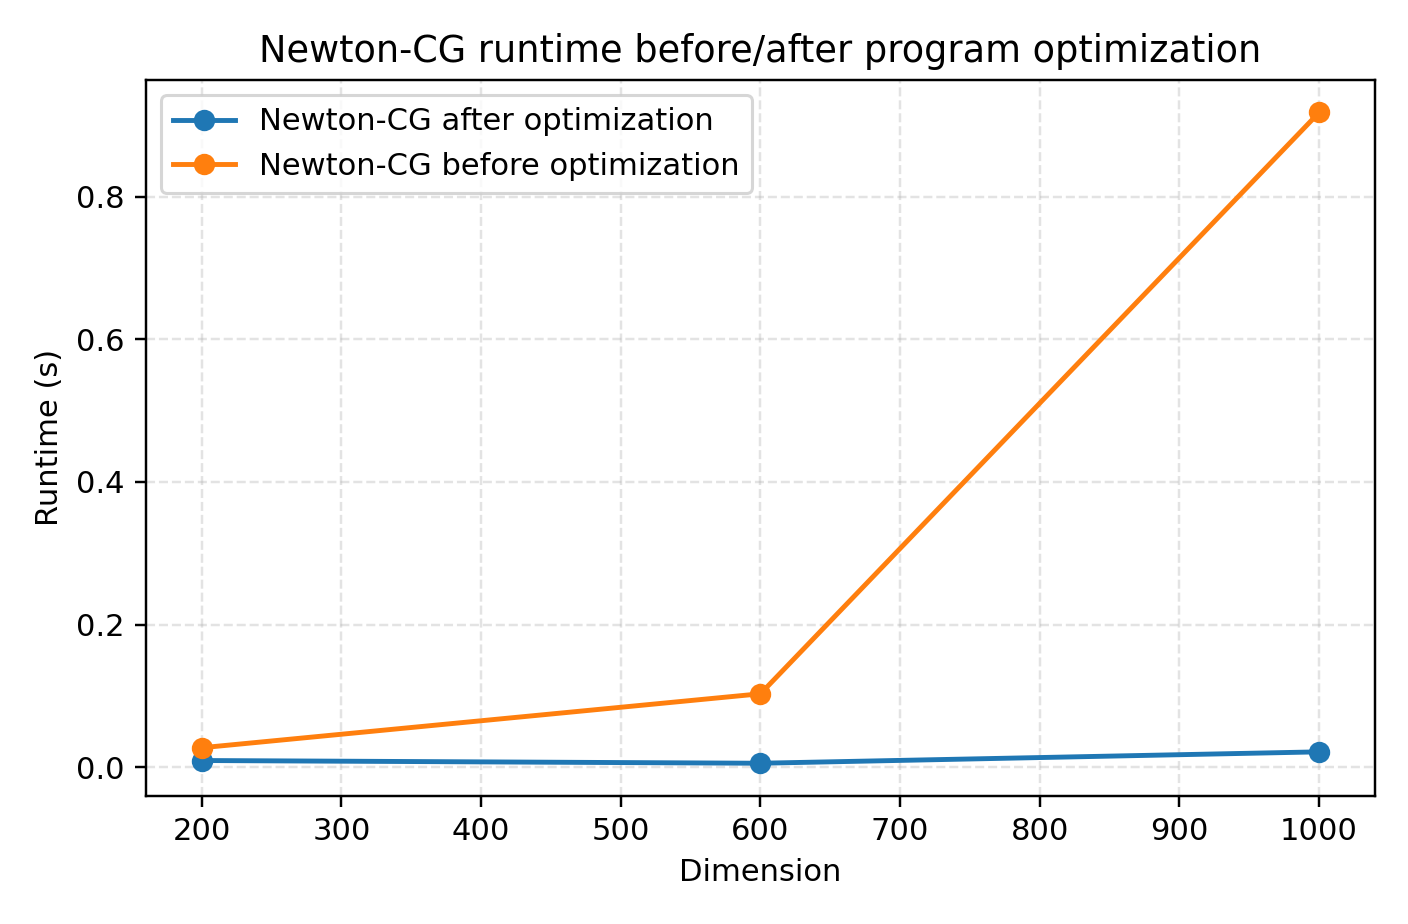
\includegraphics[width=0.72\linewidth]{work4_newton_cg_optimization_runtime.png}
\caption{Newton-CG 在程序优化前后的运行时间曲线}
\label{fig:work4-opt-runtime}
\end{figure}

从表 \ref{tab:benchmark} 可以先看到一个非常明确的现象：\textbf{优化前后迭代次数完全相同，但运行时间差异很大。}
这说明本次程序优化并没有改变算法路径，也没有改变收敛结果，
它提升的纯粹是每一步计算的执行效率。

进一步看加速比：
\begin{itemize}
  \item 当 \(n=100\) 时，加速比约为 \(2.90\)；
  \item 当 \(n=300\) 时，加速比约为 \(18.40\)；
  \item 当 \(n=500\) 时，加速比约为 \(42.53\)。
\end{itemize}

随着规模增大，加速效果越来越明显。
向量化实现和 Hessian-向量积更多利用了 NumPy 的底层批量计算能力，因此规模越大越占优势。


\subsection{FR 与 Newton-CG 的比较}
在完成程序优化后，我再用优化版目标函数对 FR 和 Newton-CG 做主实验比较。
结果如表 \ref{tab:maincompare} 所示。

\begin{table}[H]
\centering
\caption{FR 与 Newton-CG 在扩展 Rosenbrock 上的比较结果}
\label{tab:maincompare}
\begin{tabular}{ccccccc}
\toprule
\(n\) & 方法 & 运行时间/s & 迭代次数 & \(f^\ast\) & 是否收敛 & \(\|\nabla f(x^\ast)\|\) \\
\midrule
1000 & FR + Armijo & 0.04522 & 55 & \(4.70\times 10^{-11}\) & 是 & \(6.32\times 10^{-6}\) \\
1000 & Newton-CG + Armijo & 0.02697 & 19 & \(2.12\times 10^{-17}\) & 是 & \(6.09\times 10^{-8}\) \\
\midrule
10000 & FR + Armijo & 3.49834 & 158 & \(1.16\times 10^{-10}\) & 是 & \(9.58\times 10^{-6}\) \\
10000 & Newton-CG + Armijo & 0.08689 & 19 & \(2.12\times 10^{-16}\) & 是 & \(1.93\times 10^{-7}\) \\
\midrule
30000 & FR + Armijo & 3.87942 & 184 & \(6.63\times 10^{-12}\) & 是 & \(2.78\times 10^{-6}\) \\
30000 & Newton-CG + Armijo & 0.27949 & 19 & \(6.36\times 10^{-16}\) & 是 & \(3.34\times 10^{-7}\) \\
\bottomrule
\end{tabular}
\end{table}

\begin{figure}[H]
\centering
\begin{subfigure}{0.49\linewidth}
  \centering
  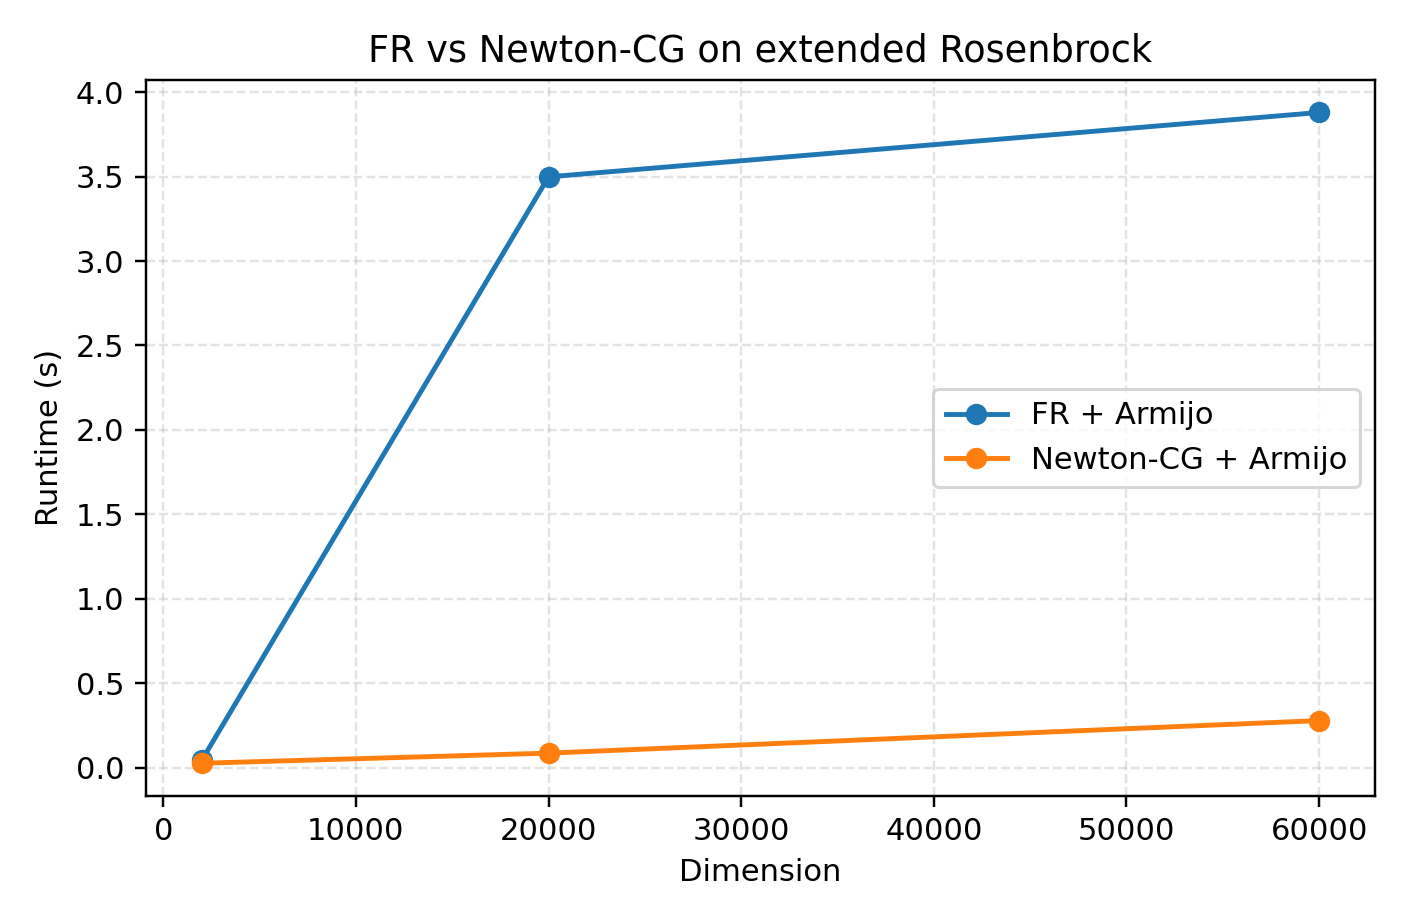
\includegraphics[width=\linewidth]{work4_method_runtime_compare.png}
  \caption{运行时间比较}
\end{subfigure}
\hfill
\begin{subfigure}{0.49\linewidth}
  \centering
  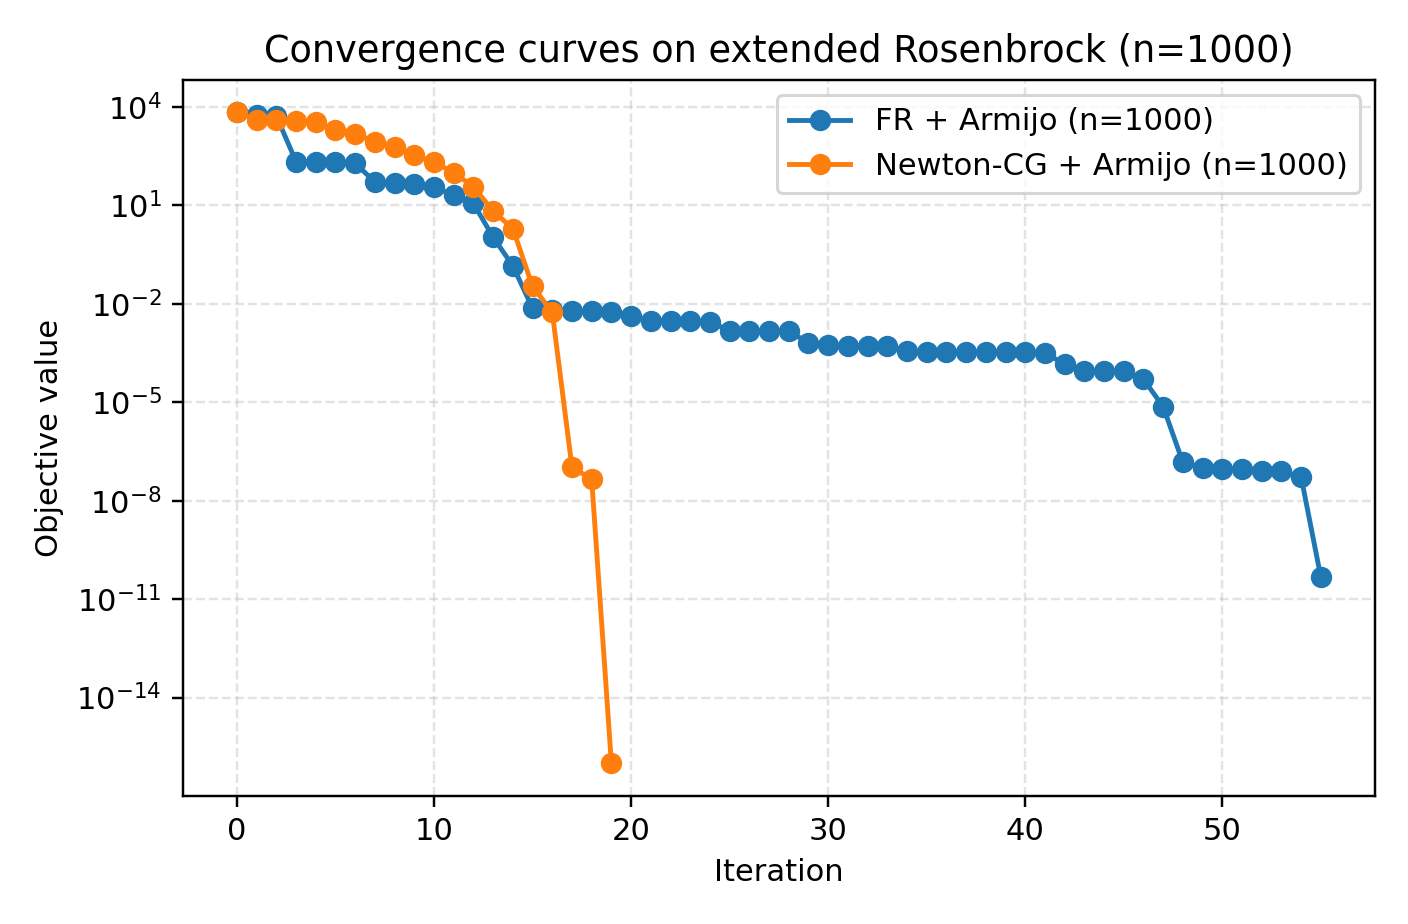
\includegraphics[width=\linewidth]{work4_convergence_curve.png}
  \caption{收敛曲线（\(n=1000\)）}
\end{subfigure}
\caption{FR 与 Newton-CG 的效率与收敛过程比较}
\label{fig:maincompare}
\end{figure}

从表 \ref{tab:maincompare} 可以得到几个比较清楚的结论。

\subsubsection*{1. 两种方法都能收敛，但 Newton-CG 收敛更快}
在三个规模下，两种算法都达到了收敛要求。
FR 作为一阶方法，虽然速度不一定快，但在这个问题上仍然是有效的。

不过从外层迭代次数看，Newton-CG 始终稳定在 \(19\) 次左右，而 FR 分别需要 \(55\)、\(158\)、\(184\) 次。
可以看出 Newton-CG 对曲率的利用更充分，能更快找到合适的下降方向。

\subsubsection*{2. Newton-CG 的时间优势在大规模下更明显}
把 FR 与 Newton-CG 的运行时间相除，可得到大致的时间加速比：
\begin{itemize}
  \item \(n=1000\) 时约为 \(1.68\)；
  \item \(n=10000\) 时约为 \(40.26\)；
  \item \(n=30000\) 时约为 \(13.88\)。
\end{itemize}

也就是说，在中大规模下，Newton-CG 比 FR 快了接近一个数量级。

\subsubsection*{3. Newton-CG 最终精度也更高}
从最终函数值和梯度范数看，Newton-CG 的结果普遍更好。
例如：
\begin{itemize}
  \item 在 \(n=10000\) 时，FR 的最终梯度范数约为 \(9.58\times 10^{-6}\)，已经接近停止阈值；
  \item 同样规模下，Newton-CG 的最终梯度范数约为 \(1.93\times 10^{-7}\)，明显更小。
\end{itemize}

这说明二阶信息不仅减少了迭代次数，也让算法更容易进入高精度区域。

\subsubsection*{4. 收敛曲线更能直观看出差异}
从图 \ref{fig:maincompare} 中 \(n=1000\) 的收敛曲线可以看到，
Newton-CG 的目标函数值下降得更陡，前十几步内就快速逼近最优值；
而 FR 的下降过程相对更慢。


\end{document}
